
\RequirePackage[l2tabu, orthodox]{nag}


\documentclass[a4paper,reqno]{amsbook}

% \usepackage[backend=biber]{biblatex}

\usepackage[pdftex,colorlinks=true]{hyperref}

\usepackage{lmodern}
\usepackage[T1]{fontenc}
\usepackage[utf8]{inputenc}
\usepackage[english]{babel}
\usepackage{microtype} %Better font spacing
%\usepackage{titlesec} %For formatting sections


\usepackage{amsmath,amssymb,amsthm,mathrsfs,latexsym,mathtools,mathdots,enumerate,tikz}


\usetikzlibrary{arrows}
\usepackage{ytableau}


\usepackage[enableskew,vcentermath]{youngtab}
\usepackage[capitalize,noabbrev]{cleveref}
\usepackage{todonotes}
\presetkeys%
    {todonotes}%
    {inline,backgroundcolor=yellow}{}


\usepackage{graphicx}

\usepackage{ifpdf}
\graphicspath{{./figures/}}
\usepackage{epstopdf}
\DeclareGraphicsExtensions{.png,.jpg,.eps,.epsf}

\newtheorem{theorem}{Theorem}
\newtheorem{proposition}[theorem]{Proposition}
\newtheorem{lemma}[theorem]{Lemma}
\newtheorem{corollary}[theorem]{Corollary}
\newtheorem{conjecture}[theorem]{Conjecture}
\newtheorem{problem}[theorem]{Problem}


\theoremstyle{definition}
\newtheorem{definition}[theorem]{Definition}
\newtheorem{example}[theorem]{Example}
\newtheorem{remark}[theorem]{Remark}

 
%  \renewcommand{\listtheoremname}{List of open problems and conjectures}


\newcommand{\defin}[1]{{\color{blue}\emph{#1}}}


\newcommand{\setN}{\mathbb{N}}
\newcommand{\setZ}{\mathbb{Z}}
\newcommand{\setQ}{\mathbb{Q}}
\newcommand{\setR}{\mathbb{R}}
\newcommand{\setC}{\mathbb{C}}
\newcommand{\setK}{\mathbb{K}}

\newcommand{\avec}{\mathbf{a}}
\newcommand{\bvec}{\mathbf{b}}
\newcommand{\pvec}{\mathbf{p}}
\newcommand{\qvec}{\mathbf{q}}
\newcommand{\rvec}{\mathbf{r}}
\newcommand{\hvec}{\mathbf{h}}
\newcommand{\xvec}{\mathbf{x}}
\newcommand{\yvec}{\mathbf{y}}
\newcommand{\zvec}{\mathbf{z}}
\newcommand{\wvec}{\mathbf{w}}
\newcommand{\uvec}{\mathbf{u}}
\newcommand{\vvec}{\mathbf{v}}
\newcommand{\svec}{\mathbf{s}}
\newcommand{\tvec}{\mathbf{t}}


\newcommand{\kappavec}{{\boldsymbol\kappa}}
\newcommand{\gammavec}{{\boldsymbol\gamma}}
\newcommand{\alphavec}{{\boldsymbol\alpha}}



%Permutations
\newcommand{\symS}{S}
\newcommand{\leqstBruhat}{\leq_{\mathrm{st}}}
\newcommand{\leqwkBruhat}{\leq_{\mathrm{wk}}}


%Polytopes
\newcommand{\polyP}{\mathcal{P}}


\newcommand{\elementary}{\mathrm{e}}
\newcommand{\monomial}{\mathrm{m}}
\newcommand{\homogeneous}{\mathrm{h}}

\newcommand{\atom}{\mathcal{A}}
\newcommand{\grothG}{\mathfrak{G}}%Grothendieck
\newcommand{\sgrothG}{\mathrm{G}} %Stable Grothendieck
\newcommand{\grothg}{\mathrm{g}}  %Dual stable  Grothendieck
\newcommand{\hlPolyP}{\mathrm{P}}
\newcommand{\hlPolyQ}{\mathrm{Q}}
\newcommand{\jackJ}{\mathrm{J}}
\newcommand{\key}{\mathcal{K}}
\newcommand{\LLT}{\mathrm{G}}
\newcommand{\macdonaldH}{\tilde{H}}
\newcommand{\macdonaldJ}{\mathrm{J}}
\newcommand{\macdonaldP}{\mathrm{P}}
\newcommand{\schubert}{\mathfrak{S}}
\newcommand{\schurS}{\mathrm{s}}
\newcommand{\schurLoop}{\mathrm{s}}
\newcommand{\qSymSchur}{\mathcal{S}}
\newcommand{\schurP}{\mathrm{P}}
\newcommand{\schurQ}{\mathrm{Q}}
\newcommand{\superS}{\mathcal{S}}


% Tableaux
\newcommand{\NAWF}{\mathrm{NAWF}}
\newcommand{\RPP}{\mathrm{RPP}}
\newcommand{\SMST}{\mathrm{SMST}}
\newcommand{\SSAF}{\mathrm{SSAF}}
\newcommand{\SSYT}{\mathrm{SSYT}}
\newcommand{\SSRT}{\mathrm{SSRT}}
\newcommand{\SYT}{\mathrm{SYT}}
\newcommand{\SVT}{\mathrm{SVT}}
\newcommand{\YT}{\mathrm{YT}}
\newcommand{\GT}{\mathrm{GT}}



% Spaces of polynomials
\newcommand{\QSYM}{\textsc{QSYM}}


% Math operators
\DeclareMathOperator{\length}{\ell}
\DeclareMathOperator{\trace}{tr}
\DeclareMathOperator{\lrmin}{lrmin}
\DeclareMathOperator{\id}{id}
\DeclareMathOperator{\height}{ht}
\DeclareMathOperator{\hook}{hook}
\DeclareMathOperator{\spin}{spin}
\DeclareMathOperator{\leg}{leg}
\DeclareMathOperator{\arm}{arm}
\DeclareMathOperator{\inv}{inv}
\DeclareMathOperator{\maj}{maj}
\DeclareMathOperator{\coinv}{coinv}
\DeclareMathOperator{\dn}{dn}
\DeclareMathOperator{\charge}{charge}


\setlength{\parskip}{0.1cm}



% \titleformat{<command>}[<shape>]{<format>}{<label>}{<sep>}{<before-code>}[<after-code>]
% \titleformat{\section}[runin]{\large}{}{0em}{}[\newline\noindent]
% \titlespacing{\section}{0pc}{1.5ex plus .1ex minus .2ex}{1pc}
% 
% \titleformat{\subsection}[runin]{\normalfont\bfseries}{}{0em}{}[\newline\noindent]
% \titlespacing{\subsection}{0pc}{1.5ex plus .1ex minus .2ex}{1pc}

%
%
% Main text in LaTeX or in HTML (or in polynomial data file)?
% How to deal with in-doc links/references?
% How to deal with overview of properties?
% References/citations?
% Background/appendix (non-polynomial topics)?
% Tableaux / figures?
% 

\newcommand{\polynomial}[1]{\section{#1}\label{ter:#1}}


\title{Symmetric polynomials and more}
\author{Per Alexandersson}
\begin{document}

\maketitle


\tableofcontents


\chapter{Classical bases}


\section{Classical bases for the space of symmetric functions}

Power-sum, elementary, complete homogeneous, monomial,
Hall inner product,


\section{Gessel fundamental basis}

This is a basis for $\QSYM$, indexed by subsets of $[n-1]$.




\chapter{Schur polynomials}

The original definition of Schur polynomials is given by the Weyl formula.

\defin{Weyl formula:}
\begin{equation}
 \schurS_\lambda(x_1,\dotsc,x_n) = \left( \prod_{1\leq i < j \leq n} (x_i-x_j) \right)^{-1}
\begin{vmatrix}
x_1^{\lambda_1+n-1} & x_2^{\lambda_1+n-1} & \dots & x_n^{\lambda_1+n-1} \\
x_1^{\lambda_2+n-2} & x_2^{\lambda_2+n-2} & \dots & x_n^{\lambda_2+n-2} \\
\vdots & \vdots & \ddots & \vdots \\
x_1^{\lambda_n} & x_2^{\lambda_n} & \dots & x_n^{\lambda_n}
\end{vmatrix}
\end{equation}

\noindent
\defin{Combinatorial definition:}

Lattice-path interpretation,
Lattice-points interpretation in Gelfand--Tsetlin polytopes.


\noindent
\defin{Jacobi--Trudi identity}

\noindent
\defin{Murighan--Nakaygama}


\noindent
\defin{Giambelli formula}





\section{Formulas for Schur polynomials}


\noindent
\defin{Cauchy identities}

\begin{equation}
 \sum_\lambda s_\lambda(x) s_{\lambda}(y) = \sum_\lambda m_\lambda(x) h_{\lambda}(y)= \prod_{i,j} \frac{1}{1-x_i y_j}.
\end{equation}
By applying $\omega$ on the $y$-alphabet, we get the second Cauchy identity
\begin{equation}
 \sum_\lambda s_\lambda(x) s_{\lambda'}(y) = \sum_\lambda m_\lambda(x) e_{\lambda}(y) = \prod_{i,j} (1+x_i y_j).
\end{equation}
% There is a finite version:
% \begin{equation}
%  \sum_{\substack{\lambda \\ \length(\lambda) \leq \min(k,m)}}
%   s_\lambda}(x_1,\dotsc,x_k) s_{\lambda}(y_1,\dotsc,y_m) = \prod_{i=1}^k \prod_{j=1}^m (1-x_i y_j)^{-1}
% \end{equation}

\noindent
\defin{Littlewood-Richardson rule}

\noindent
\defin{Pieri rule} Special case of the Littlewood--Richardson rule.


\defin{Robinson--Schenstedt--Knuth correspondence (RSK)}



\section{Open problems and conjectures}

\begin{conjecture}
Let $\lambda \geq \mu$ in domination order. Show that for every non-negative vector $\xvec \geq 0$ in $\setR^n$,
\begin{equation}
 \frac{\schurS_\lambda(\xvec)}{\schurS_\lambda(1,\dotsc,1)} \geq \frac{\schurS_\mu(\xvec)}{\schurS_\mu(1,\dotsc,1)}.
\end{equation}
This appears in \emph{Inequalities for Symmetric Means}, by Cuttler, Greene and Skandera.
See \url{http://www.lehigh.edu/~mas906/papers/smean11-18.pdf}.

Note: This is proved in \url{http://arxiv.org/abs/1502.04753}.
\end{conjecture}


\begin{problem}
Note that multiplication of Schur polynomials can be seen as a Minkovski sum of GT-polytopes,
which motivates the question:
Is there a lifting of the Littlewood--Richardson rule to lattice points in GT-polytopes?
\end{problem}



Skew Schur polynomials expands positively in the Gessel fundamental quasi-symmetric functions,
\[
\schurS_{\lambda/\mu} = \sum_{T \in \SYT(\lambda/\mu)} F_{D(T)}
\]
where $D(T)$ is the descent set of $T$.



\chapter{Other variants of Schur polynomials}


\polynomial{Schur polynomial (flagged)}


Let $\phi$ be a weakly increasing sequence (flag) of positive integers.
The \defin{flagged skew Schur polynomial} is defined as
\begin{equation}
\schurS_{\lambda/\mu}(\xvec) = \sum_{T \in \SSYT(\lambda/\mu,\phi)} x^T
\end{equation}
where the sum is over all semi-standard Young tableaux of shape $\lambda/\mu$
and the entries in row $i$ do not exceed $\phi_i$.
Gessel--Viennot--Lindelöf give the Jacobi--Trudi identity
\begin{equation}
\schurS_{\lambda/\mu}(\xvec) = \det(h_{\lambda_i-\mu_j-i+j}(\xvec_{\phi_i}))_{1\leq i,j \leq n}
\end{equation}
where $\xvec_l = (x_1,\dots,x_l)$.

There is a flagged Littlewood--Richardson rule, that expresses flagged skew Schur polynomials
as a non-negative sum of key polynomials, see \cite{ReinerShimozono1995}.
% TODO: That paper (V. Reiner, M. Shimonzo) has lots of other stuff on key polys.



\polynomial{Schur polynomial (symplectic and orthogonal)}

%See  symplectic-and-orthogonal-schur-hamel0267.pdf

These have Giambelli-type formulas.



\polynomial{Schur polynomial (cylindric)}

% See definition in
% http://www-igm.univ-mlv.fr/~fpsac/FPSAC05/ARTICLES/P21.pdf


\polynomial{Schur polynomial (affine)}


\polynomial{Schur polynomial (loop)}


\todo{Define the space these polynomials live in.}

Fix a natural number $r \in \setN$. Given a box $s=(i,j)$ in a skew SSYT $T$,
we define the weight as $w(s) \coloneqq x_{T(s)}^{c(s)}$, where the ``mirror'' content $\bar{c}(s)$
is defined as $\bar{c}(s) = i-j \in \setZ/r\setZ$.
The weight $\xvec^T$ of a tableau is as usual the product of the weights of the boxes.

% Taken from https://arxiv.org/pdf/0812.0840.pdf
\begin{align}\label{eq:schurLoopDefinition}
\schurLoop_{\lambda/\mu}^{(r)}(\xvec) \coloneqq \sum_{T \in \SSYT(\lambda/\mu)} \xvec^T
\end{align}
At $r=1$, we recover the usual Schur functions. These functions live in $LSym^{(r)}$, the space of loop symmetric functions.
Define the loop variants of the elementary and homogeneous symmetric functions as
\begin{align}
\elementary_{k}^{(r)}(x_1,\dotsc,x_m) \coloneqq \sum_{1\leq i_1 < i_2 < \dotsb < i_k \leq m} x_{i_1}^{(r)} x_{i_2}^{(r+1)} \dotsm x_{i_k}^{(r+k-1)}
\end{align}
and
\begin{align}
\homogeneous_{k}^{(r)}(x_1,\dotsc,x_m) \coloneqq \sum_{m\geq i_1 \geq i_2 \geq \dotsb \geq i_k \geq 1} x_{i_1}^{(r)} x_{i_2}^{(r+1)} \dotsm x_{i_k}^{(r+k-1)}.
\end{align}
These are also in the space of $LSym^{(r)}$.


%From https://arxiv.org/pdf/1504.03782.pdf
We have the identities
\begin{align}
 \schurLoop_{(k)}^{(r)} = h_k^{(r-k+1)} \qquad \text{and} \qquad \schurLoop_{(1^k)}^{(r)} = h_k^{(r)}.
\end{align}
\begin{proposition}[Loop Jacobi--Trudi]
For $\lambda$ with at most $m$ parts, we have
\begin{align}
 \schurLoop_{\lambda}^{(r)}(x_1,\dotsc,x_m) = [ \homogeneous_{\lambda_i - i + j}^{(r-\lambda_i+j)}].
\end{align}
\end{proposition}

There is an analogue of the Weyl formula, expressing the loop Schur function
as a ratio of alternants. %see  https://arxiv.org/pdf/1504.03782.pdf

% There is a cylindrical version of these, see
% https://arxiv.org/pdf/1607.03232.pdf


% There is a loop power-sum symmetric function, and also a loop Murighan--Nakaygama rule,
% see  https://arxiv.org/pdf/1504.03782.pdf



\polynomial{Schur polynomial (modular)}


\polynomial{Schur polynomial (non-commutative)}
%there are two versions according to Stanley, EC2, p. 417



\polynomial{Schur polynomial (non-symmetric)}


\polynomial{Schur polynomial (P and Q)}

% See \url{http://www.ams.org/journals/tran/2013-365-02/S0002-9947-2012-05653-4/S0002-9947-2012-05653-4.pdf}

% Certain skew schur functions are schur-p positive.
% https://www.researchgate.net/publication/51930445_Staircase_skew_Schur_functions_are_Schur_P-positive

The Schur $\schurP$ functions are obtained by specializing $t=-1$ for the Hall--Littlewood polynomials,
$\schurP_\lambda(\xvec)=\hlPolyP_\lambda(\xvec;-1)$.

There is a combinatorial formula for $\schurP_\lambda$ whenever $\lambda$ is strict.
\begin{equation}
\schurP_\lambda(\xvec) = \sum_{T \in \SMST(\lambda)} \xvec^{T}
\end{equation}
where $\SMST(\lambda)$ is the set of semi-standard marked shifted tableaux of shape $\lambda$.

They are a basis for the subring of symmetric functions, $\setQ[p_1,p_3,p_5,\dotsc]$, generated by the odd power-sum functions.


\begin{definition}
A  semi-standard marked shifted tableau of shape $\lambda$ is a filling of a shifted tableau,
with the alphabet $\{1'<1<2'<2<\dotsb\}$, such that
\begin{enumerate}
\item Entries are weakly increasing along rows and columns,
\item each row contains at most one marked entry,
\item each column contains at most one marked entry,
\item and there is no marked entry on the main diagonal.
\end{enumerate}
The weight do not distinguish marked and non-marked entries.
\end{definition}


\medskip
Stembridge gives the following Schur expansion.
Let $U$ be a fixed SYT of shape $\lambda$.
Then
\begin{align}
 \schurP_\lambda = \sum_{\substack{T \in SYT(\cdot) \\ \mathrm{jdt}(T) = U}} \schurS_{sh(T)}
\end{align}
where $\mathrm{jdt}(T)$ is the \emph{shifted jeu de taquin} rectification.


\medskip
Stembridge gives a Littlewood--Richardson rule for the Schur $\schurP$ functions.


\medskip 

The Schur $\schurQ$ polynomials are multiples of the Schur $\schurP$ polynomials:
\begin{align*}
\schurQ_\lambda(\xvec) =
\begin{cases}
2^{\length(\lambda)} \schurP_\lambda(\xvec) &\text{ if $\lambda$ is strict}, \\
0 &\text{ otherwise}
\end{cases}
\end{align*}


Define an inner product $[p_\lambda,p_\mu] = z_\lambda \delta_{\lambda\mu} 2^{-\length(\lambda)}$.
Then the Schur-$P$ and Schur-$Q$ functions are dual --- $[\schurP_\lambda,\schurQ_\mu] = \delta_{\lambda \mu}$.

We have the Cauchy type identity
\[
 \sum_{\lambda \in DP} \schurQ_\lambda(\xvec)\schurP_\lambda(\yvec) = \prod_{i,j} \frac{1+x_iy_j}{1-x_iy_j}
\]
where $DP$ is the set of partitions with \emph{distinct} parts (that is, strict).


There is a Littlewood--Richardson rule, (and a crystal proof in \url{https://arxiv.org/pdf/1706.09969.pdf})
\[
 \schurQ_{\lambda/\mu}(\xvec) = \sum_{\nu} f^{\nu}_{\lambda,\mu} \schurQ_\nu(\xvec).
\]




\polynomial{Schur polynomial (skew)}

\polynomial{Schur polynomial (ribbon)}
These are a special case of skew Schur polynomials, where the shape is a ribbon.
Expands positively in Schur polynomials, see \cite{Haglund2011463}.






\polynomial{Schur polynomial (double/factorial)}




Let $T$ be a semistandard tableau, and let $(\xvec|\yvec)^T$ be defined as
\[
 (\xvec|\yvec)^T = \prod_{(i,j) \in T} (x_{T(i,j)} + y_{T(i,j) + j-i}).
\]
The \defin{double Schur polynomials} are defined as
\begin{equation}
\schurS_{\lambda/\mu}(\xvec||\yvec) = \sum_{T \in \SSYT(\lambda/\mu)} (\xvec|\yvec)^T. 
\end{equation}



% Are these same as Schur superpolynomials? Probably not..
% See 6th variation in Macdonalds overview also.
\polynomial{Schur polynomial (super)}

% NOTE- COMPARE WITH MOLEV -- THESE ARE MORE OR LESS DOUBLE SCHUR FUNCTIONS!

The \defin{super Schur polynomials} are also known as \emph{hook Schur functions} or \emph{supersymmetric Schur functions},
are 

A super semi-standard Young tableau is a filling of a shape $\lambda$ with the alphabet
$1<2<3<\dotsb < \overline{1}< \overline{2}< \overline{3}<\dotsb$.
such that the unbarred entries form a filling of some $\nu \subseteq \lambda$,
\begin{enumerate}
\item rows and columns are weakly increasing,
\item the unbarred entries are strictly increasing in columns,
\item the barred entries are strictly increased in rows.
\end{enumerate}
Then
\begin{equation}
\superS_\lambda(\xvec,\yvec) = \sum_{T \in \SSYT(\lambda)} x^T y^{\overline{T}}
\end{equation}
where the sum is over all super-fillings of $\lambda$,
 and the weight $x^T$ only considers the unbarred entries, and $y^{\overline{T}}$ only consider the barred entries.

\medskip


Let $\lambda$ be a partition with $\ell$ parts. Then the super Schur functions can be defined as
\begin{equation}
\superS_\lambda(\xvec,\yvec) = \det_{1\leq i,j \leq \ell} (h_{\lambda_i -i +j}(\xvec,\yvec))
\text{ where } \sum_{m\geq 0} h_m(\xvec, \yvec) z^m = \frac{ \prod_{i \in \setZ } (1+y_i z)}{ \prod_{j \in \setZ} (1-x_jz)  }.
\end{equation}
This formula is due to Pragacz and Thorup. There is also a skew version,
\begin{equation}
\superS_{\lambda/\mu}(\xvec,\yvec) = \det_{1\leq i,j \leq \ell} (h_{\lambda_i-\mu_j - i +j}(\xvec,\yvec)).
\end{equation}

\medskip 


% See Krattenthaler, 1272-1351-1-PB.pdf

These have a determinant formula, Cauchy formula and  Jeu-de-Taquin.



\polynomial{Schur polynomial (shifted)}

\[
\schurS^\star_\mu (x_1,\dotsc,x_n)
= \frac {\det \left( (x_i+n-i)_{\mu_j+n-j} \right)}
{\det \left( (x_i+n-i)_{n-j} \right)}
\]
Special case of the factorial Schur polynomials.



We define the \defin{shifted Schur polynomials} $\schurS^{\#}_\mu(\xvec)$ as
\begin{equation}
\schurS^{\#}_\mu(\xvec) = \sum_{T \in RSSYT} \prod_{s \in \mu} (x_{T(s)} -  \arm'(s) + \leg'(s)),
\label{EqOkounkovCombJsh}
\end{equation}
where $\arm'(s) = j-1$ and $\leg'(s) = i-1$ for the box $s=(i,j)$. Thus, the top degree component of 
$\schurS^{\#}_\mu$ is given by the ordinary Schur function $\schurS_\mu$.

These are the unique polynomials that satisfy the vanishing conditions
\begin{equation}\label{eq:vanishing}
\schurS^{\#}_\mu(\lambda) =
\begin{cases}
H_\mu,   &\lambda = \mu \\
0, \quad &|\mu| \leq |\lambda|, \; \mu \neq \lambda.
\end{cases}
\end{equation}
where $H_\lambda$ is the product of hooks, $\prod_{s \in \lambda} (\arm_\lambda(s) + \leg_\lambda(s) + 1)$.


\url{https://arxiv.org/pdf/q-alg/9605042.pdf}


\subsection{Shifted Schur structure constants}


Define the Littlewood--Richardson type structure constants, $c^{\lambda}_{\mu\nu}$, by the relation
\[
\schurS_\mu^\# \schurS_\nu^\# = \sum_\lambda c^{\lambda}_{\mu\nu} \schurS_\lambda^\#
\]
In particular, if $|\lambda|=|\mu|+|\nu|$, then $c^{\lambda}_{\mu\nu}(\alpha)$ coincide with the usual Littlewood--Richardson coefficients.
From the vanishing result (see \cite[top of page 4434]{MolevSaganLRFactorialSchur}), it follows that
$c^{\lambda}_{\mu\nu}$ is identically zero unless $\lambda \supseteq \mu$ and $\lambda \supseteq \nu$. 



\subsection{A recursion formula for $c^{\lambda}_{\mu\nu}$}

We start with a small proposition, that give a simple formula for $c^{\lambda}_{\mu \lambda}$:
\begin{proposition}
We have that $c^{\lambda}_{\mu \lambda} = \schurS^{\#}_\mu(\lambda)$.
\end{proposition}
\begin{proof}
This follows from evaluating the definition of $c^{\lambda}_{\mu \lambda}$ in $\lambda$:
\[
\schurS_\mu^\#(\lambda) \schurS_\lambda^\#(\lambda) = \sum_\rho c^{\rho}_{\mu\lambda} \schurS_\rho^\#(\lambda).
\]
Now using the vanishing condition in \eqref{eq:vanishing}, we see that only the term $\rho = \lambda$
survives and from this we can easily deduce the statement.
\end{proof}


\begin{proposition} \label{prop:structureConstantRecursion}
Let $\mu, \nu \subseteq \lambda$. Then
\begin{equation}
c^{\lambda}_{\mu\nu} = 
\frac{1}{|\lambda|-|\nu|}\left( 
 \sum_{\nu \to \nu^+} c^{\lambda}_{\mu \nu^+} -
 \sum_{\lambda^- \to \lambda } c^{\lambda^-}_{\mu \nu}
\right)
\end{equation}
where the first sum is taken over all possible ways to add one box to the diagram $\nu$,
and the second sum is over all ways to remove one box from $\lambda$.
\end{proposition}
This together with the identity $c^{\lambda}_{\mu \lambda} = \schurS^{\#}_\mu(\lambda)$
gives a method to compute the $c^{\lambda}_{\mu\nu}$.



\begin{problem}
The Littlewood-Richardson coefficient $c^{\lambda}_{\mu,\nu}$ may be obtained as a Kronecker coefficient:
\[
c^{\lambda}_{\mu,\nu} =  g( (n-|\lambda|, \lambda),  (n-|\mu|, \mu), (n-|\nu|, \nu) ),
\]
for $n$ sufficiently large. Is there a similar specialization in the case $|\mu|+|\nu|\neq |\lambda|$?

Note that the above formula does not immediately generalize, $c_{(2),(1)}^{(2)} = 2$, but $g((4,2),(5,1),(4,2))=1$. 
\end{problem}



\chapter{Grothendieck and Schubert polynomials}



\section{Grothendieck polynomial}

See \url{https://arxiv.org/pdf/math/0405539.pdf} for some nice formulas, as chains in bruhat order, etc.


\subsection{Double Grothendieck polynomials}

There is also an operator definition of the more
general Grothendieck polynomials --- these are indexed by permutations and similar to the Schubert polynomials
and introduced by Lascoux and Schützenberger in 1982.


Let $\omega_0 = n\,(n-1)\,\dotsc 2 \, 1$ be the longest permutation in $\symS_n$. Define
\begin{equation}
\grothG_{\omega_0}(\xvec,\yvec) = \prod_{i+j \leq n} (x_i+y_j-x_i y_j)
\end{equation}
and define
\begin{equation}
\grothG_{\omega} = \pi_i \grothG_{\omega s_i}
\end{equation}
whenever $\length(\omega s_i) = \length(\omega) + 1$ and where $\pi_i$ is the \defin{isobaric divided difference operator}
\[
 \pi_i(f) = (1-x_{i+1}) \partial_i(f) =  \frac{ (1-x_{i+1})f - (1-x_{i}) s_i f }{ x_i-x_{i+1} }.
\]

The Grothendieck polynomials have an analogue of Monk's formula, see \url{http://www.math.tamu.edu/~sottile/research/pdf/Grothendieck.pdf}.


% See Macnamara, there is a \beta-parameter that should be present.
%
%

The \defin{stable Grothendieck polynomials} are defined via the limit
\begin{equation}
\sgrothG_\omega(\xvec,\yvec) = \lim_{n \to \infty} \grothG_{1^n \times \omega}(\xvec,\yvec).
\end{equation}
This is analogous to how the Stanley symmetric functions are the stable limit of Schubert polynomials.


\subsection{Stable Grothendieck polynomials}

%
% % Littlewood-Richardson rule given in A. S. Buch,
% A Littlewood-Richardson Rule for the
% K
% -Theory of Grassmannians
% ,
% Acta. Math,
% 189
% (2002), 37–78

The stable \defin{Grothendieck polynomials} $\sgrothG_\lambda(\xvec)$ can be defined (see \cite{Buch2002}) as
\begin{equation}
 \sgrothG_\lambda(\xvec) = \sum_{T \in \SVT(\lambda)} (-1)^{|T|-|\lambda|}x^{w(T)}
\end{equation}
where the sum is taken over \defin{set-valued Young tableaux}. These are defined as
fillings of a diagram of shape $\lambda$, but now each box contains a \emph{set} of natural numbers.
For two such sets $A$, $B$ we have $A<B$ if $\max A < \min B$ and similar for $A \leq B$.
With this notation, $\SVT(\lambda)$ is the set of all set-valued tableaux (subsets of $[n]$) such that rows are weakly increasing,
and columns are strictly increasing. Here, the $i$th component of $w(T)$ is now the total number of sets where $i$ appears,
and $|T|$ is the sum over all cardinalities of the sets in the boxes.
Note that the lowest-degree part of $\sgrothG_\lambda(\xvec)$ is the usual Schur polynomial $\schurS_\lambda(\xvec)$.

There is also a skew version.

They have a Cauchy identity, see \url{http://www.math.tamu.edu/~sottile/research/pdf/Grothendieck.pdf}
There is a finite Cauchy identity, see \url{https://arxiv.org/pdf/1604.00104.pdf}

There are factorial (stable)  Grothendieck polynomials, see \url{http://math.stanford.edu/~petermc/fgparxivfinal.pdf} and 
\url{http://arxiv.org/pdf/math/0508192v2.pdf}. These have a LR-rule.


\section{Grothendieck polynomial (dual)}

\begin{equation}
\grothg_\lambda(\xvec) = \sum_{T \in \RPP(\lambda)} x^{ev(T)}
\end{equation}
Here, $ev(T)$ is the composition where the $i$th component denotes the total number of columns of $T$ containing $i$.

The highest degree term of $\grothg_\lambda(\xvec)$ is given by the Schur polynomial $\schurS_\lambda$.

Let $f^\lambda_\mu$ be the number of \defin{elegant fillings} of the skew shape $\lambda/\mu$.
A filling is elegant if rows are weakly increasing, columns are strictly increasing
and the numbers in row $i$ are in $[i-1]$.
\begin{theorem}[Lam, Pylyavskyy, \cite{Lam07combinatorialhopf}]
Let $\lambda$ be a partition. Then
\begin{equation}
 \grothg_\lambda(\xvec) = \sum_{\mu \subseteq \lambda} f^\lambda_\mu \schurS_\mu.
\end{equation}
\end{theorem}




\section{Schubert polynomial}

Indexed by permutations.
\[
 \schubert_\omega(\xvec) =  \partial_{(w^{-1}w_0)} x_1^{n-1}x_2^{n-2}\dotsm x_{n-1}^{1}
\]


\section{Schubert polynomial (double)}

For Grassmann permutations, these are the factorial/double Schur polynomials.
See \url{http://sporadic.stanford.edu/bump/factorial.pdf}




\section{Stanley symmetric functions}

These have non-negative integer expansions in terms of Schur polynomials.

% 


\chapter{Hall--Littlewood and Jack polynomials}


\section{Hall--Littlewood polynomial}

The Hall--Littlewood $\hlPolyP$ polynomials may be defined as
\begin{equation}\label{eq:HallLittlewoodPDefinition}
\hlPolyP_\lambda(\xvec;t) = \left( \prod_{i\geq 0} \prod_{j=1}^{m_\lambda(i)} \frac{1-t}{1-t^{j}} \right)
\sum_{\sigma \in \symS_n} \sigma\left(   x_1^{\lambda_1}\dotsm x_n^{\lambda_n} \prod_{i<j} \frac{x_i - tx_j}{x_i-x_j}     \right),
\end{equation}
where $\lambda = (\lambda_1,\dotsc,\lambda_n)$, some parts might be zero and $m_\lambda(i)$ denotes the number of parts of $\lambda$ equal to $i$
and $\sigma$ acts on the indexing of the variables. Note that it is important to take the number of parts equal to zero in consideration.
\medskip


The Hall--Littlewood $\hlPolyP$ polynomials interpolates between the Schur polynomials and the monomial symmetric functions,
\[
 \hlPolyP_\lambda(\xvec;0) = \schurS_\lambda(\xvec), \qquad \hlPolyP_\lambda(\xvec;1) = \monomial_\lambda(\xvec).
\]
Note that \cref{eq:HallLittlewoodPDefinition} reduces to the Weyl formula when $t=0$.

\medskip 

The Hall--Littlewood $\hlPolyQ$ polynomials interpolates between the Schur polynomials and the complete homogeneous symmetric functions.
\todo{Make definition here.}
% Using a different normalization, one obtains the Hall--Littlewood $Q$ polynomials as
% \begin{equation}\label{eq:HallLittlewoodQDefinition}
% \hlPolyQ_\lambda(\xvec;t) = \frac{(1-t)^{\length(\lambda)}}{ \prod_{i=1}^{n-l} \frac{1-t^i}{1-t} }
% \sum_{\sigma \in \symS_n} \sigma\left(   x_1^{\lambda_1}\dotsm x_n^{\lambda_n} \prod_{i<j} \frac{x_i - tx_j}{x_i-x_j}     \right),
% \end{equation}


The specialization $\hlPolyQ(\xvec,-1)$ is the Schur-$P$ function.

\medskip


The \defin{Kostka--Foulkes} polynomials are defined via the relation
\[
\schurS_\lambda(\xvec) = \sum_\mu K_{\lambda \mu}(t) \hlPolyP_\mu(\xvec; t)
\]

The \defin{modified Hall--Littlewood polynomials} may be defined via $\hlPolyQ'_\mu((1-t)\xvec; t) = \hlPolyQ_\mu(\xvec; t)$
\[
\hlPolyQ'_\mu(\xvec; t) = \sum_\lambda K_{\lambda \mu}(t)\schurS_\lambda(\xvec)
\]

Lascoux and Schützenberger proved that
\[
  K_{\lambda \mu}(t) = \sum_{T \in \SSYT(\lambda, \mu)} t^{\charge(T)}.
\]


% These have a combinatorial interpretation of the multiplicative structure constants,
% see http://arxiv.org/pdf/math/0506287v3.pdf

% There are polytope interpretations: http://arxiv.org/pdf/1505.04269.pdf


\section{Hall--Littlewood polynomial (non-symmetric)}

\todo[inline]{Rewrite, fix notation}

In \cite{Haglund2011463}, a \defin{non-symmetric} analogue of Hall--Littlewood polynomials are defined,
indexed by weak integer compositions.

Let $\NAWF(\alpha)$ denote the set of all non-attacking augmented fillings of shape $\alpha$ with
weakly decreasing rows and basement given by $\beta_i =i$.
The non-symmetric, integral form Hall--Littlewood polynomials, $\hlPolyP_\alpha(x_1,\dots,x_n)$, may be defined as
\begin{equation}
\hlPolyP_\alpha(\xvec;t) = \sum_{T \in \NAWF(\alpha) } \xvec^{w(T)} t^{\coinv(T)} (1-t)^{\dn(T)}
\end{equation}
where $\coinv(T)$ is the number of triples in $T$ which are \emph{not} inversion triples,
and $\dn(T)$ is the number of pairs of adjacent boxes, $(i,j)$ and $(i,j+1)$ such that $T(i,j) \neq T(i,j+1)$ (different neighbors). 
They show that the ordinary Hall--Littlewood polynomials expands in terms of these non-symmetric Hall--Littlewood polynomials.
\[
 \hlPolyP_\mu(\xvec;t) = \sum_{\substack{\alpha\\ \lambda(\alpha) = \mu}} \hlPolyP_\alpha(\xvec;t).
\]
% 
% It is possible to define a Kostka--Foulkes polynomial analogue in this case, where we expand the key polynomials
% in terms of the non-symmetric Hall--Littlewood polynomials:
% \begin{equation}
% \key_\alpha(\xvec) = \sum_{\beta} K_{\alpha\beta}(t) \hlPolyP_\beta(\xvec;t).
% \end{equation}
% 
% \begin{problem}
% Show that $K_{\alpha\beta}(t) \in \setN[t]$.
% \end{problem}
% This has been verified by computer for $\length(\alpha)\leq 6$ and $|\alpha| \leq 9$.
% 
% \begin{example}
% \[
% \key_{152}(\xvec) = \hlPolyP_{251}(\xvec;t) + t \hlPolyP_{341}(\xvec;t) + t \hlPolyP_{431}(\xvec;t) + \hlPolyP_{521}(\xvec;t)
% \]
% \end{example}


\section{Jack polynomials}

The \defin{Jack polynomials} are deformations of the Schur polynomials.


\defin{Knop--Sahi formula}

\begin{equation}
 \sum_{\lambda} \frac{\jackJ_\lambda(x)\jackJ_\lambda(y)}{}
\end{equation}



\defin{Jack polynomial (shifted)}


\defin{Jack polynomial (non-symmetric)}


Double Jack, see \url{http://www.emis.de/journals/SIGMA/2015/051/sigma15-051.pdf}



\polynomial{Zonal spherical function}

These are special cases of Jack polynomials, for $\alpha=2$.



\section{LLT polynomials}

The LLT polynomials $\LLT_{\lambda/\mu}^{(n)}(\xvec,q)$
are defined as
\begin{equation}
 \LLT_{\lambda/\mu}^{(n)}(\xvec,q) = \sum_{T \in n-\SSRT(\lambda/\mu)} q^{\spin(T)}x^T
\end{equation}
where the sum is taken over all $n$-ribbon semi-standard Young tableaux of shape $\lambda/\mu$.



%https://math.berkeley.edu/~mhaiman/ftp/jim-conjecture/formula.pdf
% The LLT-polynomials can be defined as
% \[
%  G_\lambda(\xvec,q) = \sum_{T \in SSYT(\lambda)} q^{\inv(T)} \xvec^T
% \]
% where two boxes $u$, $v$, form an \emph{inversion} if
% \begin{enumerate}
%  \item $T(u) < T(v)$
% \end{enumerate}

Haiman and Grojnovski gives a representation-theoretical proof that LLT-polynomials are Schur-positive,
but there is no combinatorial formula for the coefficients in the expansion.


\chapter{Macdonald polynomials}


\polynomial{Macdonald polynomial}



The Macdonald polynomials specialize to the Hall--Littlewood $\hlPolyP$ polynomials and the Schur polynomials:
\[
\macdonaldP_\mu(\xvec;0,t)= \hlPolyP(\xvec;t), \quad
\macdonaldP_\mu(\xvec;q,q)= \schurS_\mu(\xvec), \quad
\macdonaldP_\mu(\xvec;q,1) = \monomial_\mu(\xvec), \quad
\lim_{t \to 1} \macdonaldP_\mu(\xvec; t^\alpha,t) = \jackJ_\mu (\xvec; \alpha)
\]

The $\macdonaldJ_\mu(\xvec;q,t)$ are the \defin{integral form} Macdonald polynomials,
and we have that
\[
\macdonaldJ_\mu(\xvec;q,t) = \prod_{s \in \mu} (1-q^{\arm(s)}t^{\leg(s)+1}) \macdonaldP_\mu(\xvec;q,t).
\]

The Macdonald--Kostka polynomials are defined as 
\[
 \schurS_\lambda(\xvec) = \sum_\mu K_{\lambda\mu}(q,t) \macdonaldJ_\mu(\xvec;q,t)
\]

It is conjectured that the Macdonald polynomials $\macdonaldJ_\lambda(x,q,q^k)/(1-q)^{|\lambda|}$ are Schur-positive.

The $q,t$-Kostka polynomials are defined via the expansion in Schur functions (note the plethystic substitution)
\[
 \macdonaldJ_\mu(\xvec;q,t) = \sum_\mu K_{\lambda\mu}(q,t) \schurS_\lambda[\xvec (1-t)].
\]
Note that $K_{\lambda\mu}(0,t) = \sum_{T \in \SSYT(\lambda,\mu)} t^{\charge(T)}$.


\polynomial{Macdonald polynomial (modified)}

\begin{equation}
\macdonaldH_\mu(\xvec;q,t) = \sum_{T \in YT(\lambda)} q^{\inv(T)}t^{\maj(T)}\xvec^T
\end{equation}


The \defin{modified $qt$-Kostka coefficients} are defined as
\begin{equation}
\macdonaldH_\mu(\xvec;q,t) = \sum_\lambda \tilde{K}_{\lambda \mu}(q,t)\schurS_\lambda(\xvec)
\end{equation}
These are related to the ordinary $qt$-Kostka polynomials via $\tilde{K}_{\lambda \mu}(q,t) = K_{\lambda \mu}(q,1/t)t^{n(\mu)}$
where $n(\mu)$ is the sum of the leg-lengths in the diagram $\mu$.

It is known that $\tilde{K}_{\lambda \mu}(q,t) \in \setN[q,t]$, but an open problem
to give a combinatorial description of these.


\todo[inline]{

It is conjectured that the Macdonald poly, $\macdonaldJ_\lambda(x,q,q^k)/(1-q)^{|\lambda|}$ is Schur-positive.
  
Plethystic subst. for non-sym polys is $x_i^k \mapsto x_i^k(1-t^k)$?
}


\polynomial{Macdonald polynomial (non-symmetric)}

\todo{Explain the different notations.}

\polynomial{Macdonald polynomial (non-homogeneous)}





\chapter{Demazure atoms and key polynomials}

In this section, we give the combinatorial background
needed to define the key polynomials and Demazure atoms.


\section{Augmented fillings}

Let $\beta = (\beta_1,\dots,\beta_n)$ be a list of $n$ different positive integers
and let $\alpha=(\alpha_1,\dots,\alpha_n)$ be a weak integer composition, that is, a vector with non-negative integer entries.
An \defin{augmented filling} of shape $\alpha$ and \emph{basement} $\beta$
is a filling of a Young diagram of shape $(\alpha_1,\dotsc,\alpha_n)$ with positive integers,
augmented with a zeroth column filled from top to bottom with $\beta_1,\dotsc,\beta_n$.


\begin{definition}
Let $T$ be an augmented filling. Two boxes $a$, $b$, are \defin{attacking}
if $T(a)=T(b)$ and the boxes are either in the same column, or they are in adjacent columns, with the rightmost box in a row strictly below the other box.
\begin{align*}
\begin{ytableau}
a  \\
\none[\scriptstyle\vdots] \\
b  \\
\end{ytableau}\quad
\text{or}\quad
\begin{ytableau}
 a & \none \\
 \none[\scriptstyle\vdots] \\
  & b \\
\end{ytableau}
\end{align*}
\end{definition}
A filling is \defin{non-attacking} if there are no attacking pairs of boxes.


\begin{definition}
Let $T$ be an augmented filling. A \defin{descent} in $T$ is a box $(i,j)$ such that $T(i,j-1) < T(i,j)$.
\end{definition}


\begin{definition}
A \defin{triple of type $A$} is an arrangement of boxes, $a$, $b$, $c$,
located such that $a$ is immediately to the left of $b$, and $c$ is somewhere below $b$,
and the row containing $a$ and $b$ is at least as long as the row containing $c$.

Similarly, a \defin{triple of type $B$} is an arrangement of boxes, $a$, $b$, $c$,
located such that $a$ is immediately to the left of $b$, and $c$ is somewhere above $a$,
and the row containing $a$ and $b$ is \emph{strictly} longer than the row containing $c$.


A type $A$ triple is an \defin{inversion triple} if the entries ordered increasingly,
form a \emph{counter-clockwise} orientation. Similarly, a type $B$ triple is an inversion triple
if the entries ordered increasingly form a \emph{clockwise} orientation.
If two entries are equal, the one with largest subscript in \cref{eq:invTriplets}
is considered largest.
\begin{equation}\label{eq:invTriplets}
\text{Type $A$:}\quad
\ytableausetup{centertableaux,boxsize=1.2em}
\begin{ytableau}
 a_3 & b_1 \\
 \none  & \none[\scriptstyle\vdots] \\
\none & c_2 \\
\end{ytableau}
\qquad
\text{Type $B$:}\quad
\ytableausetup{centertableaux,boxsize=1.2em}
\begin{ytableau}
c_2 & \none \\
\none[\scriptstyle\vdots]  & \none \\
a_3 & b_1 \\
\end{ytableau}
\end{equation}
\end{definition}


\begin{example}
The bold entries are descents, and the underlined entries form a type $A$ inversion triple.
There are $7$ inversion triples (of type $A$ and $B$) in total.
\[
\begin{ytableau}
\underline{4} & \underline{2} & 1 & \textbf{2} & 4\\
5 & 5\\
3 & 3 & \textbf{4} & 3\\
2\\
1 & \underline{1} \\
\end{ytableau}
\]
\end{example}


\todo{What is called arm here is called leg in other places. Argh...}
The \defin{major index}, $\maj(T)$, of an augmented filling $T$ is given by
\[
\maj(T) = \sum_{\substack{ s \in T \\ a \text{ is a decent}}} \arm(s)+1
\]
where $\arm(s)$ is the number of boxes to the right of $s$.
The \emph{number of inversions}, $\inv(T)$ of a filling is the number of inversion triples of either type.
The number of coinversions, $\coinv(T)$, is the number of type $A$ and type $B$ triples that are \emph{not}
inversion triples.



\subsection{Semi-standard augmented fillings}

A \defin{semi-standard augmented filling}, ($\SSAF$) of \emph{shape} $\alpha$ and \emph{basement} $\beta$
is an augmented filling of shape $\alpha$ and basement $\beta$ with weakly decreasing rows and every triple is an inversion triple.
Note that this definition implies that there are no attacking boxes in an $\SSAF$.
In particular, all entries in every column are different.


The \defin{weight} $w(T)$ of an augmented filling is given by the vector where the $i$th
coordinate counts the number of entries excluding basement in $T$, which are equal to $i$.
\begin{example}\label{ex:generalAtomFilling}
Here is an example of a semi-standard augmented filling, with basement $(1,3,2,5,4)$.
\[
\ytableausetup{centertableaux,boxsize=1.2em}
\begin{ytableau}
\mathbf{1} & \none \\
\mathbf{3} & 3 & \underline{1} & 1 \\
\mathbf{2} & 2 \\
\mathbf{5} & 5 & 5 & 5\\
\mathbf{4} & 4 & \underline{4} & \underline{3} & 2
\end{ytableau}
\]
We can for example check the underlined entries for the type $B$ inversion triple condition --- since
$1$, $3$ and $4$ are oriented in a clockwise manner, they form an inversion triple.
The weight is given by $(2,2,2,2,3)$.
\end{example}


Let $\SSAF_\beta(\alpha)$ denote all semi-standard augmented fillings with basement $\beta$ and shape $\alpha$.
We define the \defin{general Demazure atoms} $\atom^\beta_\alpha(\xvec)$ as the polynomials
\begin{equation}
\atom^\beta_\alpha(\xvec) = \sum_{T \in \SSAF_\beta(\alpha)} \xvec^{w(T)}.
\end{equation}
In particular, the \defin{atom} $\atom_\alpha(\xvec)$ and the \defin{key polynomial} $\key_\alpha(\xvec)$
are defined as
\[
\atom_\alpha(\xvec) = \atom^{(12\dotsc n)}_\alpha(\xvec) \text{ and } \key_\alpha(\xvec) = \atom^{(n \dotsc 21)}_\alpha(\xvec).
\]


\begin{remark}
 Note that some authors define the key polynomial $\key_\alpha(\xvec)$ as the sum over fillings with the reversed shape,
for example in the paper ``Refinements of the Littlewood--Richardson rule''.
\end{remark}


\subsection{Demazure operators}

The key polynomials and atoms can be defined via \defin{divided difference operators}.
Let $s_i$ denote the transposition $(i,i+1)$ and let such
transpositions act on $\setZ[x_1,\dotsc,]$ by permuting the indices of the variables.
Define the divided difference operators
\[
 \partial_i = \frac{1-s_i}{x_i-x_{i+1}}, \quad \pi_i = \partial_i x_i, \quad \theta_i = \pi_i -1.
\]
Given a permutation $\omega \in \symS_n$, let $\omega = s_{i_1}\dotsm s_{i_l}$
be expressed via a reduced word $i_1i_2\dots i_l$.
Then, let $\pi_\omega = \pi_{i_1}\dotsm \pi_{i_l}$ and $\theta_\omega = \theta_{i_1}\dotsm \theta_{i_l}$.
It can be shown that these operators does not depend on the choice of the reduced word.
Furthermore, let $\omega_0 \in \symS_n$ denote the unique permutation with length $\binom{n}{2}$.
Remember that $\omega_0$ applied to a list reverses the order of the entries in the list.

To apply $\pi_\omega = \pi_{i_1}\dotsm \pi_{i_l}$ to a polynomial $p(\xvec)$,
we simply compute $p(\xvec) \pi_{i_1}$ and apply $\pi_{i_2} \dotsm \pi_{i_{l}}$ recursively.
The key polynomial indexed by $\omega$ and $\lambda$ may now be defined (see \cite{ReinerShimozono1995}) as $\key_{\omega,\lambda}(\xvec)  = \xvec^{\lambda} \pi_{\omega}$.
It turns out that
\[
 \key_{\omega,\lambda}(\xvec) = \key_\alpha(\xvec) = \atom^\omega_\lambda(\xvec)
\]
where $\lambda$ is the partition obtained by sorting the parts of $\alpha$ in decreasing order
and $\omega$ is the \emph{shortest} permutation such that $\omega \omega_0(\lambda) = \alpha$.
That this indeed is equivalent to the definition above was proved in \cite{Mason2009}.
In a similar fashion, the Demazure atoms $\atom_{\omega,\lambda}(\xvec)$ are defined as $\xvec^\lambda \theta_{\omega}$,
and
\[
 \atom_{\omega,\lambda}(\xvec) = \atom_\alpha(\xvec)
\]
where $\lambda$ is the partition obtained by sorting the parts of $\alpha$ in decreasing order
and $\omega$ is a shortest permutation such that $\omega(\bar{\lambda}) = \alpha$.


\begin{example}
Let $\alpha=(2,0,2,1,3)$ and $\lambda=(3,2,2,1,0)$.
Then taking $\omega=s_3s_2s_4$ we see that $\omega\omega_0(\lambda) = \omega(0,1,2,2,3)$ which simplifies to $\alpha$.
We now compute the key polynomial $\key_{20213}(\xvec)$ with the operator definition.
First $\xvec^\lambda = x_1^3x_2^2x_3^2x_4$, so we have
\begin{align*}
(x_1^3x_2^2x_3^2x_4) \pi_3 \pi_2 \pi_4  &= (x_1^3 x_2^2 x_3^2 x_4+x_1^3 x_2^2 x_3 x_4^2) \pi_2 \pi_4 \\
&= (x_1^3 x_2^2 x_3^2 x_4+x_1^3 x_2^2 x_3 x_4^2+x_1^3 x_2 x_3^2 x_4^2)\pi_4 \\
&= x_1^3 x_2^2 x_3^2 x_4+x_1^3 x_2^2 x_3 x_4^2+x_1^3 x_2 x_3^2 x_4^2+x_1^3 x_2^2 x_3^2x_5 \\
&\phantom{=} +x_1^3 x_2^2 x_3 x_4 x_5+x_1^3 x_2 x_3^2 x_4 x_5+x_1^3 x_2^2 x_3 x_5^2+x_1^3 x_2x_3^2 x_5^2.
\end{align*}

One can also obtain $\key_{20213}(\xvec)$ from semi-standard augmented fillings of $\alpha$:
\begin{align*}
\begin{ytableau}
5 & 4 & 3\\
4\\
3 & 3 & 2\\
2 & 2\\
1 & 1 & 1 & 1\\
\end{ytableau}
\quad
\begin{ytableau}
5 & 4 & 4\\
4\\
3 & 3 & 2\\
2 & 2\\
1 & 1 & 1 & 1\\
\end{ytableau}
\quad
\begin{ytableau}
5 & 4 & 4\\
4\\
3 & 3 & 3\\
2 & 2\\
1 & 1 & 1 & 1\\
\end{ytableau}
\quad
\begin{ytableau}
5 & 5 & 3\\
4\\
3 & 3 & 2\\
2 & 2\\
1 & 1 & 1 & 1\\
\end{ytableau} \\
%
\begin{ytableau}
5 & 5 & 4\\
4\\
3 & 3 & 2\\
2 & 2\\
1 & 1 & 1 & 1\\
\end{ytableau}
\quad
\begin{ytableau}
5 & 5 & 4\\
4\\
3 & 3 & 3\\
2 & 2\\
1 & 1 & 1 & 1\\
\end{ytableau}
\quad
\begin{ytableau}
5 & 5 & 5\\
4\\
3 & 3 & 2\\
2 & 2\\
1 & 1 & 1 & 1\\
\end{ytableau}
\quad
\begin{ytableau}
5 & 5 & 5\\
4\\
3 & 3 & 3\\
2 & 2\\
1 & 1 & 1 & 1\\
\end{ytableau}
\end{align*}
\end{example}


\todo[inline]{Make an atom example}

\begin{proposition}[CITE SMTH]
Let $\lambda$ be a partition and $\omega$ a permutation. Then
\begin{equation}
\key_{\omega,\lambda}(\xvec) = \sum_{\omega' \leqstBruhat \omega} \atom_{\omega',\lambda}(\xvec).
\end{equation}
Using Möbius inversion, it follows that
\begin{equation}
\atom_{\omega,\lambda}(\xvec) = \sum_{\omega' \leqstBruhat \omega} (-1)^{\ell(\omega)-\ell(\omega')}\key_{\omega',\lambda}(\xvec).
\end{equation}
\end{proposition}



\subsection{The key polynomials from Kogan faces}

In \cite{Kiritchenko2010}, it was proven that key polynomials
can be expressed as a kind of the integer point transform of a union of Kogan faces of a Gelfand--Tsetlin polytope.
Let $\GT(\lambda,\omega) \subseteq \GT(\lambda)$ be the union of all \emph{reduced} Kogan faces with type $\omega$.

\begin{theorem}[See \cite{Kiritchenko2010}]
Let $\omega \in \symS_n$ and $\lambda$ be a partition. Then
\begin{align*}
\key_{\omega(\lambda)}(\xvec) &= \sum_{G \in \GT(\lambda,\omega)} \xvec^{w(G)} \\
\key_{\omega,\lambda}(\xvec) &= \sum_{G \in \GT(\lambda,\omega_0\omega^{-1})} \xvec^{w(G)}.
\end{align*}
\end{theorem}

It is now clear that we can express the Demazure atoms as
\begin{equation}
\atom_{\omega,\lambda}(\xvec) = \sum_{\omega' \leqstBruhat \omega} (-1)^{\ell(\omega)-\ell(\omega')} \sum_{G \in \GT(\lambda,\omega_0\omega^{-1})} \xvec^{w(G)}.
\end{equation}
Using \cref{lemma:rkfInclusion} together with the second identity, we can ``lift'' this identity to the lattice points in
the GT-polytope $\GT(\lambda)$.

We probably end up with a formula of the form
\begin{theorem}
\begin{equation}
\atom_{\omega,\lambda}(\xvec) = \sum_{G \in \GT(\lambda) : \sigma(G)=\omega } \xvec^{w(G)}
\end{equation}
\end{theorem}
where $\sigma(G)$ is some statistic. This will most certainly be the same as having the ``right key'' as in Lascoux definition.


\todo[inline]{There is something  called composition arrays, which are similar to GT-patterns,
that also generate key polys....
}

%
% \begin{lemma}
% If $\omega' \leq \omega$ in the weak Bruhat order, then $\GT(\lambda,\omega) \subseteq \GT(\lambda,\omega')$.
% \end{lemma}
% \begin{proof}
% Assume that $G$ is a point in $\GT(\lambda,\omega)$.
% Then $G$ is in some reduced Kogan face and $\omega = s_{i_1}\dotsm s_{i_l}$ where the transpositions are given by the equalities.
% Since $\omega' \leq \omega$ we know that $\omega'$ can be expressed as a reduced subword\todo{Is this true?} of $\omega$.
% These equalities
% \end{proof}

\subsection{Properties of atoms and key polynomials}

There is a Cauchy formula for key polynomials, see book by Lascoux:
%http://www-igm.univ-mlv.fr/~al/ARTICLES/CoursYGKM.pdf
There is a key--atom Cauchy formula, see
``An analogue of the Robinson-Schensted-Knuth
correspondence and non-symmetric Cauchy kernels for
truncated staircases''.

This is a Cauchy formula for keys and atoms.
\begin{equation*}
\prod_{\substack{i+j \leq n+1 \\ 1 \leq i , j \leq n}} (1-x_iy_j)^{-1} = \sum_{ \alpha \in \setN^n} \key_\alpha(\xvec) \atom_\alpha(\yvec)
= \sum_{ \substack{ F \in Atom \\ G \in Atom } } \xvec^F \yvec^G
\end{equation*}
where the latter sum is over all pairs of atom fillings.

\begin{problem}
 Find a Cauchy formula involving atoms with general basements.
\end{problem}




The atoms have a Murighan-Nakaygama rule. %http://www.dmtcs.org/pdfpapers/dmAS0182.pdf
This generalizes to generalized Demazure atoms, with the type B condition.


\todo[inline]{
Key times Schubert does not expand positively in keys, and sometimes not at all.
Ex: Schubert{1,3,2}, and key{1,0,1} gives a -1 in the expansion.
}



\begin{problem}
Some problems related to skyline fillings
\begin{enumerate}
\item Are there hook formulas for skyline fillings?
\item Is there a saturation statement for key-Kostka coefficients?
\end{enumerate}
\end{problem}


\begin{problem}
Can we make a definition of key polynomials similar to that of Hall--Littlewood polynomials, (equivalent to the Weyl character formula),
as a sum over permutations?
\end{problem}



\section{Refinements of the Littlewood--Richardson rule}

In \cite{HAGLUND-RefinementsOfTheLRRule}, they show
\[
  \atom_\alpha(\xvec) \times \schurS_\lambda(\xvec) = \sum_\gamma c_{\alpha,\lambda}^\gamma \atom_\gamma(\xvec),
 \quad c_{\alpha,\beta}^\gamma \geq 0.
\]

They also prove that
\begin{equation}
\key_\alpha(\xvec) \times \schurS_\lambda(\xvec)= \sum c_{\alpha,\lambda}^\gamma \key_\gamma(\xvec), \quad c_{\alpha,\lambda}^\gamma \geq 0.
\end{equation}


The expansion of a general product $\key_\alpha(\xvec) \times \key_\beta(\xvec)$ in terms of atoms might give negative coefficients.
For example, $\key_{020}(\xvec) \cdot \key_{101}(\xvec)$ have some negative coefficients in the key expansion.

However, we have the following conjecture:
\begin{conjecture}[Key times key in atoms]
It is conjectured that
\begin{equation}
\key_\alpha(\xvec) \times \key_\beta(\xvec) = \sum_\gamma c_{\alpha,\beta}^\gamma \atom_\gamma(\xvec), \quad c_{\alpha,\beta}^\gamma \geq 0.
\end{equation}
and it is believed that a product of any number of key polynomials expands positively into atoms.
\end{conjecture}


\begin{conjecture}[Partition atom times general atom]
It is conjectured that for each basement $\beta$, we have
\begin{equation}
\atom_\lambda(\xvec) \times \atom^\beta_\alpha(\xvec) = \sum_\gamma c_{\lambda,\alpha}^\gamma \atom^\beta_\gamma(\xvec), \quad c_{\lambda,\alpha}^\gamma \geq 0.
\end{equation}
\todo[inline]{Anna is working on the case when $\beta$ is the atom basement.}
\end{conjecture}


% THERE IS A LARGER TABLE IN KeysConjectures.tex
\begin{center}
\begin{tabular}{r|cccc}
 $\times$	& $\atom_\lambda$	& $\atom_\alpha$	& $\key_\lambda = \schurS_\lambda$	& $\key_\alpha$ \\
\hline
 $\atom_\mu$	& $+\atom$		& $+\atom$	& $+\key$				& $+\key$ (crystal proof) \\
 $\atom_\gamma$	& $\cdot$		& $\times$	& $+\atom$				& $\times$\\
 $\key_\mu$	& $\cdot$		& $\cdot$	& $+\schurS$ (LR-rule)			& $+\key$\\
 $\key_\gamma$	& $\cdot$		& $\cdot$	& $\cdot$				& $+\atom$?
\end{tabular}
\end{center}


Note that $+\schurS \Rightarrow +\key \Rightarrow +\atom$.
\todo{Include general basement atom}



\section{Quasi-symmetric Schur polynomials}


Indexed by integer compositions.

Schur polynomials expands positively in quasi-symmetric Schur polynomials.
Hence, these expands positively in terms of Demazure atoms.


There is no Littlewood--Richardson rule for quasisymmetric Schur polynomials in general,
but there is one in the following special case:
\begin{equation}
\schurS_\lambda \times \qSymSchur_\alpha = \sum c^\beta_{\alpha\lambda} \qSymSchur_\beta
\end{equation}
with non-negative $c^\beta_{\alpha\lambda}$.









\chapter{List of unsolved problems}

\begin{itemize}

 \item Schubert structure constants (Littlewood--Richardson generalization)
 \item Kronecker coefficients (Littlewood--Richardson generalization)
 \item (Shifted Jack) structure constants positivity (Littlewood--Richardson generalization)
 \item Find a combinatorial formula for the plethystic substitution $\langle \schurS_\lambda[\schurS_\mu], \schurS_\nu \rangle$.

 \item Modified Macdonald into Schur. Follows from LLT into Schur.
 \item LLT into Schur (Littlewood--Richardson and charge generalization)
 \item $q$-Chromatic symmetric function into elementary.
 \item $q$-Chromatic symmetric function into Schur (bijective proof).

\item Find a Knop--Sahi formula for non-homogeneous Jack polynomials.

 \item Key times key into atoms
 \item Key into t-atoms (charge generalization)
 \item q-key into key (charge generalization)
 \item Skew-atoms into atoms (Littlewood--Richardson generalization)
 \item Fixed descent atoms into atoms
 \item Jacobi--Trudi for keys.
 
 \item Katabolic Hall--Littlewood into Schur, see p. 81 in \url{https://arxiv.org/pdf/1301.3569.pdf}.
 
 \item Haglunds plethystic Schur into Schur $\schurS_\lambda[\xvec/(1-z)]$ into $\schurS_\mu(\xvec)$ (with a normalization).
 

 \item Is $k \to \key_{k\alpha}(1^n)$ a polynomial with non-negative coefficients? These polynomials
 are specializations of Demazure polynomials, see doi:10.1016/j.jalgebra.2006.07.002
 \item Is $k \to c^{k\lambda}_{k\mu,k\nu}$ a polynomial with non-negative coefficients?
\end{itemize}



\chapter{Other stuff (WIP)}

\defin{Heckmann--Opdam operator}


\defin{Dimer model}

\defin{Falling factorial}
The falling factorial, $(x)_k$ is defined as $x(x-1)(x-2)\dotsm(x-k+1)$.

\defin{Parking function}

\defin{$n$-ribbon tableau}
\defin{Set-valued tableau}

$k$-Schur, $p$-Schur, $q$-Schur,


Rigged configurations, KR-crystals, K-theory, permutahedron, associahedron, Fuss, Lah,
Mahonian statistic, Schubert variety, flag (vector spaces).
Affine flag variety, Bruhat decomposition, Borel subgroup, Schubert cell, Weyl group

Cluster algebra, Fermionic formula, cyclic sieving phenomena.
Quivers, permutation patterns




\chapter*{Appendix I: Permutations, tableaux and GT-patterns}


\section{Permutations}


\subsection{Rothe diagram}


\subsection{Maj, inv and charge}

\begin{problem}[Symmetric permutation statistics]
Is there a statistic $\sigma$ on permutations, such that
\[
\sum_{\pi \in \symS_n} q^{\inv \pi} t^{\maj \pi} r^{\sigma(\pi)}
\]
is symmetric in $q$, $t$, and $r$?

% $\sum_{\pi \in \symS_n} q^{\inv \pi} t^{\maj \pi}s^{\charge \pi} r^{\sigma(\pi)}$
\end{problem}


\subsection{Reduced words, the weak order and the Bruhat order}


A \defin{reduced word} of a permutation $\pi$ is a product of transpositions, $s_{i_1}\dotsm s_{i_\ell}$
which is equal to $\pi$, and where $\ell$ has minimal length. The reduced word is in general not unique.

The \defin{length of a permutation}, $\length(\pi)$, is the length of the reduced word,
or equivalently, the number of inversions of the permutation.


The permutation $\pi_1$ is less than $\pi_2$ if $\pi_1$ is ``more sorted'', in the sense of transpositions.


The covering relations for the \defin{left weak Bruhat order} is given by $u \gtrdot_L v$ if $u=s_iv$
and $\length(u) = \length(v)+1$. Similarly, the \defin{right weak Bruhat order} is given by $u \gtrdot_R v$ if $u=vs_i$.
Both of these are called the \defin{weak Bruhat order}, and these orderings are isomorphic under $w \to w^{-1}$.

\medskip

The \defin{strong Bruhat order} contains more relations. We have that $u >_B v$
if there are reduced words $w_u$ and $w_v$ such that $w_v$ is a subword of $w_u$.
It is clear from the definition that $u >_B v$ if and only if $u^{-1} >_B v^{-1}$.
One can show that $u \gtrdot_B v$ if there is a transposition $t$ (not necessarily simple),
such that $u = tv$, or equivalently, $u = vt'$.



\begin{figure}[!ht]
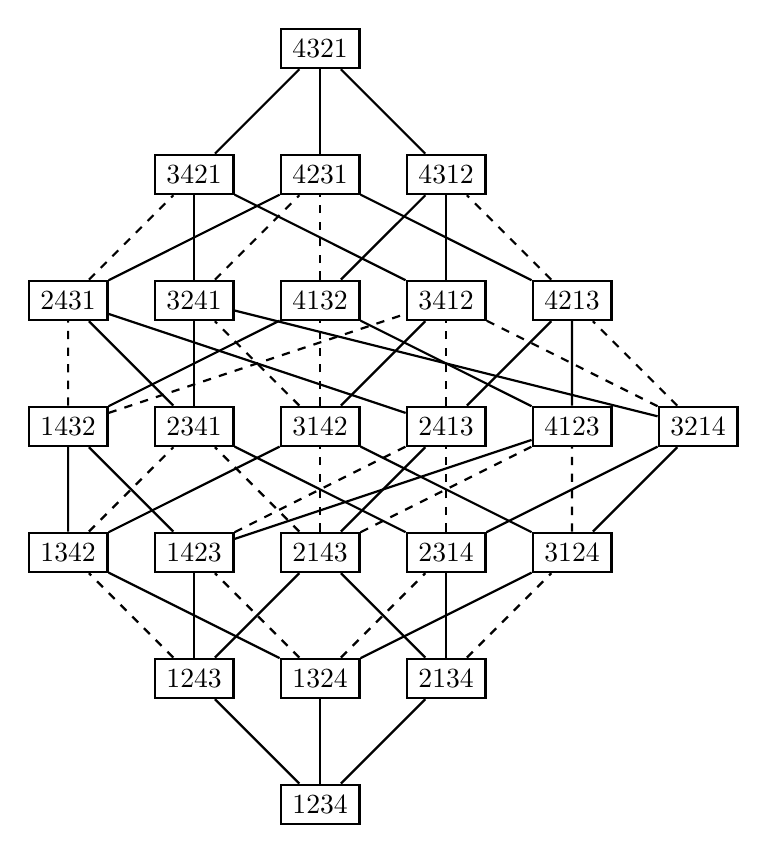
\begin{tikzpicture}[thick,scale=0.4,yscale=-1,
every node/.style = {
shape= rectangle,
draw,                    %% here
minimum width  = 1cm,
minimum height = 0.5cm,
align          = center,
text           = black},
black edge/.style  = { -,
thick,
black,
shorten >= 4pt}
]
\node (n1234) at (0.,24.) {1234};
\node (n1243) at (-4.,20.) {1243};
\node (n1324) at (0.,20.) {1324};
\node (n1342) at (-8.,16.) {1342};
\node (n1423) at (-4.,16.) {1423};
\node (n1432) at (-8.,12.) {1432};
\node (n2134) at (4.,20.) {2134};
\node (n2143) at (0.,16.) {2143};
\node (n2314) at (4.,16.) {2314};
\node (n2341) at (-4.,12.) {2341};
\node (n2413) at (4.,12.) {2413};
\node (n2431) at (-8.,8.) {2431};
\node (n3124) at (8.,16.) {3124};
\node (n3142) at (0.,12.) {3142};
\node (n3214) at (12.,12.) {3214};
\node (n3241) at (-4.,8.) {3241};
\node (n3412) at (4.,8.) {3412};
\node (n3421) at (-4.,4.) {3421};
\node (n4123) at (8.,12.) {4123};
\node (n4132) at (0.,8.) {4132};
\node (n4213) at (8.,8.) {4213};
\node (n4231) at (0.,4.) {4231};
\node (n4312) at (4.,4.) {4312};
\node (n4321) at (0.,0.) {4321};
%
\draw(n1234)-- (n1243);
\draw(n1234)-- (n1324);
\draw(n1234)-- (n2134);
\draw[dashed] (n1243)-- (n1342);
\draw(n1243)-- (n1423);
\draw(n1243)-- (n2143);
\draw(n1324)-- (n1342);
\draw[dashed] (n1324)-- (n1423);
\draw[dashed] (n1324)-- (n2314);
\draw(n1324)-- (n3124);
\draw(n1342)-- (n1432);
\draw[dashed] (n1342)-- (n2341);
\draw(n1342)-- (n3142);
\draw(n1423)-- (n1432);
\draw[dashed] (n1423)-- (n2413);
\draw(n1423)-- (n4123);
\draw[dashed] (n1432)-- (n2431);
\draw[dashed] (n1432)-- (n3412);
\draw(n1432)-- (n4132);
\draw(n2134)-- (n2143);
\draw(n2134)-- (n2314);
\draw[dashed] (n2134)-- (n3124);
\draw[dashed] (n2143)-- (n2341);
\draw(n2143)-- (n2413);
\draw[dashed] (n2143)-- (n3142);
\draw[dashed] (n2143)-- (n4123);
\draw(n2314)-- (n2341);
\draw[dashed] (n2314)-- (n2413);
\draw(n2314)-- (n3214);
\draw(n2341)-- (n2431);
\draw(n2341)-- (n3241);
\draw(n2413)-- (n2431);
\draw[dashed] (n2413)-- (n3412);
\draw(n2413)-- (n4213);
\draw[dashed] (n2431)-- (n3421);
\draw(n2431)-- (n4231);
\draw(n3124)-- (n3142);
\draw(n3124)-- (n3214);
\draw[dashed] (n3124)-- (n4123);
\draw[dashed] (n3142)-- (n3241);
\draw(n3142)-- (n3412);
\draw[dashed] (n3142)-- (n4132);
\draw(n3214)-- (n3241);
\draw[dashed] (n3214)-- (n3412);
\draw[dashed] (n3214)-- (n4213);
\draw(n3241)-- (n3421);
\draw[dashed] (n3241)-- (n4231);
\draw(n3412)-- (n3421);
\draw(n3412)-- (n4312);
\draw(n3421)-- (n4321);
\draw(n4123)-- (n4132);
\draw(n4123)-- (n4213);
\draw[dashed] (n4132)-- (n4231);
\draw(n4132)-- (n4312);
\draw(n4213)-- (n4231);
\draw[dashed] (n4213)-- (n4312);
\draw(n4231)-- (n4321);
\draw(n4312)-- (n4321);
%
\end{tikzpicture}
\caption{The weak order and the Bruhat order}\label{fig:weakAndBruhatOrder}
\end{figure}


\subsection{Wiring diagram}
This is used to represent reduced words of a permutation.



\section{Partitions and compositions}


\defin{Com\'et code}

\defin{Core partition}



\section{Young tableaux and Gelfand--Tsetlin patterns}



\subsection{Hook formulas}


The \defin{Hook formula} is a formula for computing the number of standard Young tableaux of a partition shape.
\begin{equation}
f^\lambda = \frac{|\lambda|!}{\prod_{s \in \lambda} \hook(s)}
\end{equation}
It can be seen as counting linear extensions of certain posets,
and there are generalizations of this formula to other families of posets.
The hook formula can be seen as a special case of the \emph{hook-content} formula.

There is a $q$-analogue of this, and there are generalizations to other types of posets (trees, forests, d-complete posets).

\bigskip

The \defin{Hook-content formula}



\section{Gelfand--Tsetlin patterns}

An important object related to the combinatorics of Young tableaux are the
\defin{Gelfand-Tsetlin patterns}, or GT-patterns for short.
Such a pattern is a triangular (or parallelogram) arrangement of non-negative integers:
\[
\begin{array}{cccccccccccccc}
x_{n1} & & x_{n2} & & \cdots & & \cdots & & x_{nn} \\
 & \ddots & & \ddots &  & &   & \iddots &   \\
%   &  & x_{13} &  & x_{23}  &  & x_{33}   &  & \\
   &  &  &   &   &   &     &  & \\
   & &  &   x_{21} &  & x_{22}  \\
   & &  &    & x_{11}
\end{array}
\]
The entries must satisfy the conditions
\begin{equation}
x_{i+1,j} \geq x_{ij} \text{ and } x_{ij} \geq x_{i+1,j+1} \label{eq:gtinequalities}
\end{equation}
for all values of $i$, $j$ where the indexing is defined.
The inequalities simply states that horizontal rows are weakly decreasing,
down-right diagonals are weakly decreasing and down-left diagonals are weakly increasing.

The conditions ensures every row in the pattern defines an integer partition.
Furthermore, any two adjacent rows define a skew shape.
These properties enables us to define the bijection with Young tableaux ---
the skew shape defined by row $j$ and $j+1$ in a GT-pattern $G$
describes which boxes in a tableau $T$ that have content $j$.
In particular, if $T$ has shape $\lambda$, then the topmost row is $\lambda$.
See Figure \ref{fig:gtexample} for an example of this correspondence.
\begin{figure}[!ht]
\centering
\setcounter{MaxMatrixCols}{20}
\begin{equation}\label{eq:triangulargt}
\begin{matrix}
5 &   & 4 &   & 2 &   & 1 &   & 1 &  & 0\\
 & 5 &   & 3 &   & 2 &   & 1 &   & 0\\
 &  & 3 &   & 3 &   & 2 &   & 1  \\
 &  &  & 3 &   & 3 &   & 1 &  \\
 &  &  &  & 3 &   & 2 &  \\
 &  &  &  &  & 3 & \\
\end{matrix}
\quad
\longleftrightarrow
\quad
\young(11155,2236,34,4,6)
\end{equation}
\caption{The GT-pattern corresponding to a Young tableau.
For example, the third row, $(3,3,1)$ tells us that the shape of the entries $\leq 3$ in the tableau has this shape.
}\label{fig:gtexample}
\end{figure}

Note that in any GT-pattern, $x_{i+1,j} - x_{i,j}$ counts the number of
boxes with content $i$ in row $j$ in the corresponding tableau.
The \defin{weight} $w$ of an integer GT-pattern is the weight of the corresponding Young tableau.



\section{Gelfand--Tsetlin polytopes}

Given a shape $\lambda$, the \defin{Gelfand-Tsetlin polytope}
$\polyP_{\lambda} \subset \setR^{n(n-1)/2}$ (or GT-polytope),
is defined as the convex polytope consisting of all GT-patterns $(x^i_j)_{1\leq j \leq i \leq n}$,
where we now allow real entries, that satisfy that the top row is given by $\lambda$.
The integer lattice points in this polytope are of course the
integer Gelfand--Tsetlin patterns with shape $\lambda$.

\begin{problem}
Is it NP-complete to determine if a GT-polytope has a non-integral vertex?
\end{problem}

\begin{problem}
Consider a statistic $\sigma: \SSYT \to \setN$ which satisfies $\sigma(kT) = k\sigma(T)$ for all $T$,
such as charge. Using the latter relation, we can evaluate $\sigma$ on any rational point in a GT-polytope.

For which classical statistics $\sigma$ is the extension to rational points continuous?
What is the average statistic over the GT-polytope?
\end{problem}


%
% For reference what a Gelfand-Tsetlin-polytope (GT-polytope) is [see this nice article.][1]
%
% Given partitions $\lambda$, $\mu$ of same size, we can determine if the Kostka number $K_{\lambda\mu}$ is non-zero or not in polynomial time.
% However, [computing the actual Kostka coefficient][2] is $\#P$.
%
% This translates to that determining if a GT-polytope is non-empty or not is easy, but counting lattice points inside is hard.
%
% It is also known that for a general polytope, represented as a collection of linear equalities and inequalities, it is NP-complete to determine if it has a vertex with non-integer coordinates.
% It is also NP-complete to determine if a general polytope is non-empty.
%
% The above shows that GT-polytopes are "easier" than general polytopes,
% when it comes to determining if they are non-empty, but counting lattice points is just as hard as the general case.
%
% **Now, is it still NP-complete to determine if a GT-polytope has a non-integral vertex?**
%
%
%   [1]: http://arxiv.org/abs/math/0309329
%   [2]: http://www.mit.edu/~har/kostka.pdf


\subsection{Reduced Kogan faces}

By imposing some extra equalities on the coordinates of a GT-polytope, one can obtain faces of the polytope.
There is a particular interest with equalities of the form $x_{ij}=x_{i,j+1}$.
By imposing a set of such equalities, we obtain a \defin{Kogan face} of the GT-polytope.
To each equality of the form $x_{ij}=x_{i,j+1}$, we associate the transposition $s_{n-i+j-1}$,
as shown in \cref{fig:reducedKoganFace}.
We then construct a word from these transpositions by reading the entries from bottom to top, left to right.
If this word is \emph{reduced}, we say that the corresponding Kogan face is reduced.
Note that the same word might be constructed from equalities in several different ways.
The \defin{type of a Kogan face} is the permutation obtained from the word.
\begin{figure}[!ht]
\centering
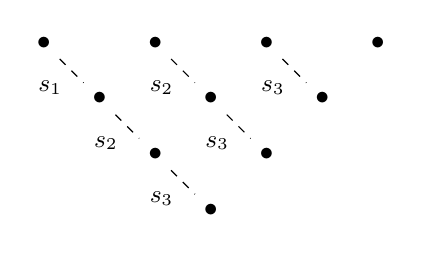
\begin{tikzpicture}
\node (N11) at (0,0) {$\bullet$};
\node [below right of=N11] (N21) {$\bullet$};
\node [above right of=N21] (N12) {$\bullet$};
\node [below right of=N12] (N22) {$\bullet$};
\node [above right of=N22] (N13) {$\bullet$};
\node [below right of=N13] (N23) {$\bullet$};
\node [above right of=N23] (N14) {$\bullet$};
\node [below right of=N21] (N31) {$\bullet$};
\node [below right of=N22] (N32) {$\bullet$};
\node [below right of=N31] (N41) {$\bullet$};

\path[-,dashed,every node/.style={font=\sffamily\small}]
(N11) edge node [below left] {$s_1$} (N21)
(N21) edge node [below left] {$s_2$} (N31)
(N31) edge node [below left] {$s_3$} (N41)
(N12) edge node [below left] {$s_2$} (N22)
(N22) edge node [below left] {$s_3$} (N32)
(N13) edge node [below left] {$s_3$} (N23);
\end{tikzpicture}
\qquad
\begin{tikzpicture}
\node (N11) at (0,0) {$\bullet$};
\node [below right of=N11] (N21) {$\bullet$};
\node [above right of=N21] (N12) {$\bullet$};
\node [below right of=N12] (N22) {$\bullet$};
\node [above right of=N22] (N13) {$\bullet$};
\node [below right of=N13] (N23) {$\bullet$};
\node [above right of=N23] (N14) {$\bullet$};
\node [below right of=N21] (N31) {$\bullet$};
\node [below right of=N22] (N32) {$\bullet$};
\node [below right of=N31] (N41) {$\bullet$};

\path[-,dashed,every node/.style={font=\sffamily\small}]
(N11) edge node [below left] {$4$} (N21)
(N21) edge node [below left] {$2$} (N31)
(N31) edge node [below left] {$1$} (N41)
(N12) edge node [below left] {$5$} (N22)
(N22) edge node [below left] {$3$} (N32)
(N13) edge node [below left] {$6$} (N23);
\end{tikzpicture}
\caption{
The transposition corresponding to different equalities between
entries in a Kogan face and the reading order of these.
}\label{fig:reducedKoganFace}
\end{figure}
We should really view the equalities that define a Kogan face as some special set of equalities ---
a point in this face might satisfy some additional equalities present, if it is also a member of some subface.
This implies that a point in th GT-polytope can be a member of \emph{several} (reduced) Kogan faces.
For example, the point with all equalities present is a member of every Kogan face.


\begin{example}
Considering the face in \cref{fig:reducedKoganFaceExample}.
All marked equalities are in the south-east direction, so we obtain the word $s_3s_1s_2s_3$.
It is straightforward to verify that this word is reduced, so this face is a reduced Kogan face.
\begin{figure}[!ht]
\centering
\begin{tikzpicture}
\node (N11) at (0,0) {$\bullet$};
\node [below right of=N11] (N21) {$\bullet$};
\node [above right of=N21] (N12) {$\bullet$};
\node [below right of=N12] (N22) {$\bullet$};
\node [above right of=N22] (N13) {$\bullet$};
\node [below right of=N13] (N23) {$\bullet$};
\node [above right of=N23] (N14) {$\bullet$};
\node [below right of=N21] (N31) {$\bullet$};
\node [below right of=N22] (N32) {$\bullet$};
\node [below right of=N31] (N41) {$\bullet$};

\path[-,dashed,every node/.style={font=\sffamily\small}]
(N11) edge node [below left] {$s_1$} (N21)
% (N21) edge node [below left] {$s_2$} (N31)
%(N31) edge node [below left] {$s_3$} (N41)
(N12) edge node [below left] {$s_2$} (N22)
(N22) edge node [below left] {$s_3$} (N32)
(N13) edge node [below left] {$s_3$} (N23);
\end{tikzpicture}
\caption{
A reduced Kogan face with the word $\omega = s_3s_1s_2s_3$.
}\label{fig:reducedKoganFaceExample}
\end{figure}

Suppose we wish to examine the GT-polytope $\polyP_\lambda$ with $\lambda=(4,3,3,2)$.
The lattice points in the reduced Kogan face with the word $s_3s_1s_2s_3$ are the following GT-patterns:
\begin{equation*}
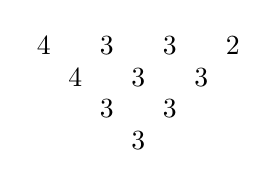
\begin{tikzpicture}[scale=0.4]
\node at (3,0) {$4$};
\node at (5,0) {$3$};
\node at (7,0) {$3$};
\node at (9,0) {$2$};
\node at (4,-1) {$4$};
\node at (6,-1) {$3$};
\node at (8,-1) {$3$};
\node at (5,-2) {$3$};
\node at (7,-2) {$3$};
\node at (6,-3) {$3$};
\end{tikzpicture}
\quad
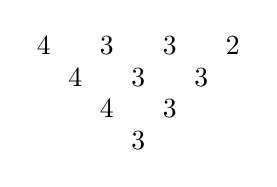
\begin{tikzpicture}[scale=0.4]
\node at (3,0) {$4$};
\node at (5,0) {$3$};
\node at (7,0) {$3$};
\node at (9,0) {$2$};
\node at (4,-1) {$4$};
\node at (6,-1) {$3$};
\node at (8,-1) {$3$};
\node at (5,-2) {$4$};
\node at (7,-2) {$3$};
\node at (6,-3) {$3$};
\end{tikzpicture}
\quad
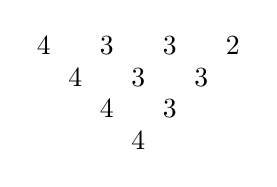
\begin{tikzpicture}[scale=0.4]
\node at (3,0) {$4$};
\node at (5,0) {$3$};
\node at (7,0) {$3$};
\node at (9,0) {$2$};
\node at (4,-1) {$4$};
\node at (6,-1) {$3$};
\node at (8,-1) {$3$};
\node at (5,-2) {$4$};
\node at (7,-2) {$3$};
\node at (6,-3) {$4$};
\end{tikzpicture}.
\end{equation*}
\end{example}


It is evident\todo{Clarify!} from the bubble-sort algorithm that there is at least one reduced Kogan face of every type $\omega \in \symS_n$.

\begin{lemma}\label{lemma:rkfInclusion}
If $F$ is a reduced  Kogan face of type $\omega$ and $\omega' \leqstBruhat \omega$ in the strong Bruhat order,
then there is a reduced Kogan face $F'$ of type $\omega'$ such that $F \subseteq F'$.
\end{lemma}
\begin{proof}
We know that $\omega$ is a reduced subword of $\omega_0 = s_n (s_{n-1} s_n) (s_{n-2} s_{n-1} s_n) \dotsm (s_1 \dotsm s_n)$,
corresponding to the word given by $F$. Now if $\omega' \leqstBruhat \omega$,
then we can express $\omega'$ as a reduced subword of $\omega$.
That reduced subword $\omega'$ is also a reduced subword of $\omega_0$, and this defines a reduced Kogan face.
\end{proof}


\todo[inline]{
There seem to be interesting stuff in the paper
``Minuscule schubert varieties: poset polytopes, pbw-degenerated demazure modules, and kogan faces''.
}

\todo[inline]{
In ``Gelfand–zetlin polytopes and Demazure characters'',
it is shown that the Ehrhart polynomial for the union of key faces
has a Hilbert-series interpretation.
}

\todo[inline]{
$132$-avoiding permutations (Kempf) are of special interest, since for each such permutation,
there is a unique Kogan face with this type.

Can we make a lattice-path model for these, and thus obtain a Jacobi-Trudi formula in this case?

This is tricky, the conditions on GT-patterns does not translate nicely to lattice paths,
such that GVL thm apply.
}


\begin{problem}
Let $a_n$ be the number of reduced Kogan faces in a GT-pattern where the top row has $n+1$ entries.
Then $a_0$, $a_1$, starts as
\[
 1,\; 2, \; 7, \; 41, \; 393, \; 6080, \; 150371, \dotsc
\]
and $a_n \leq 2^{\binom{n}{2}}$.
It would be interesting to give a formula for these integers. Note that
\[
 a_n = \#\{ \omega : \omega \text{ is a reduced subword of } s_n (s_{n-1} s_n) (s_{n-2} s_{n-1} s_n) \dotsm (s_1 \dotsm s_n) \}.
\]
This sequence is currently not in the OEIS.

Note: R. Stanley has a result on this, giving a formula for the number of reduced subwords of a specific length(?) according to Andy.

%
% Furthermore, let $rcf(\omega)$ be the number of reduced Kogan faces of type $\omega$.
% Then, $\sum_{\omega \in \symS_n} z^{rcf(\omega)}$ seem to have roots accumulating on the unit circle as $n \to \infty$.
\end{problem}

\begin{problem}
Is there some Kogan face (reduced or not) that have negative coefficients in its Ehrhart series?
Is there a reduced Kogan face whose permutation is Kempf, with negative coefficients?
The latter has some implication about key polynomials.
\end{problem}



\begin{remark}
Some Kogan faces, for example from a GT-polytope with top row $(2, 2, 2, 1, 0, 0)$ does \emph{not}
satisfy the saturation condition (when the weight is fixed, so that we have a non-integral polytope in general):
\[
%  \begin{matrix}
% 4 &   & 4 &   & 4 &   & 2\\
%  & 4 &   & 4 &   & 3 &   & 1\\
%  &  & 4 &   & 3 &   & 3 &   & 0\\
%  &  &  & 3 &   & 3 &   & 0 &   & 0\\
%  &  &  &  & 3 &   & 1 &   & 0 &   & 0\\
%  &  &  &  &  & 2 &   & 0 &   & 0 &   & 0\\
%  &  &  &  &  &  & 0 &   & 0 &   & 0 &   & 0\\
% \end{matrix}
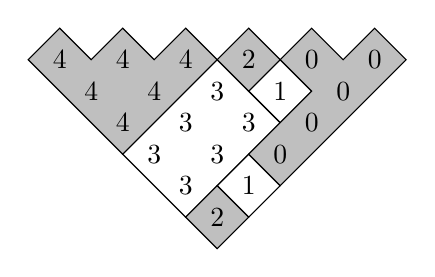
\begin{tikzpicture}[scale=0.4]
\draw[black] (8,-4)--(9,-3)--(10,-2)--(9,-1)--(8,0)--(7,-1)--(6,-2)--(5,-3)--(6,-4)--(7,-5)--(8,-4)--cycle;
\draw[black] (9,-1)--(10,-2)--(11,-1)--(10,0)--(9,-1)--cycle;
\draw[black] (8,-4)--(9,-5)--(10,-4)--(9,-3)--(8,-4)--cycle;
\filldraw[color=black,fill=lightgray] (8,0)--(9,-1)--(10,0)--(9,1)--(8,0)--cycle;
\filldraw[color=black,fill=lightgray] (7,-5)--(8,-6)--(9,-5)--(8,-4)--(7,-5)--cycle;
\filldraw[color=black,fill=lightgray] (11,-3)--(12,-2)--(13,-1)--(14,0)--(13,1)--(12,0)--(11,1)--(10,0)--(11,-1)--(10,-2)--(9,-3)--(10,-4)--(11,-3)--cycle;
\filldraw[color=black,fill=lightgray] (6,0)--(5,1)--(4,0)--(3,1)--(2,0)--(3,-1)--(4,-2)--(5,-3)--(6,-2)--(7,-1)--(8,0)--(7,1)--(6,0)--cycle;
\node at (3,0) {$4$};
\node at (5,0) {$4$};
\node at (7,0) {$4$};
\node at (9,0) {$2$};
\node at (11,0) {$0$};
\node at (13,0) {$0$};
\node at (4,-1) {$4$};
\node at (6,-1) {$4$};
\node at (8,-1) {$3$};
\node at (10,-1) {$1$};
\node at (12,-1) {$0$};
\node at (5,-2) {$4$};
\node at (7,-2) {$3$};
\node at (9,-2) {$3$};
\node at (11,-2) {$0$};
\node at (6,-3) {$3$};
\node at (8,-3) {$3$};
\node at (10,-3) {$0$};
\node at (7,-4) {$3$};
\node at (9,-4) {$1$};
\node at (8,-5) {$2$};
\end{tikzpicture}
\]
That is, we cannot change the non-shaded tiles such that all entries are even,
all entries down-left equalities are preserved and the weight vector is preserved.
\end{remark}

\begin{remark}
Note that we \emph{do} have saturation if we consider faces where equalities that should be preserved are in fixed tiles.
\end{remark}



\subsection{Pipe dream}
Also called $rc$-graphs. These are in bijection with reduced Kogan faces of GT-polytopes.
This is related to Schubert polynomials.


\subsection{Plane partitions and Lozenge tilings}


\defin{Lozenge tiling}


%Cites EVERYTING!
% \nocite{*}
\bibliographystyle{amsalpha}
\bibliography{bibliography}

\end{document}
